\documentclass[nofootinbib]{iit}%This has to remain the same

\usepackage{latexsym}% For math symbols
\usepackage[utf8]{inputenc}% Comes to rescue when non-ASCII characters are used
\usepackage[final]{graphicx}%Package for enhancement of graphics, rotation and scaling and other features 
\usepackage{lineno}
\usepackage{comment}
\usepackage{units}%Units are formatted properly
\usepackage{xfrac} %slanted fractions
\usepackage{amsmath,amsthm,amssymb,amsfonts}
\usepackage{titlesec}
\usepackage{caption}
\usepackage{subfigure}
%\usepackage[font=singlespacing,width=.98\textwidth]{subcaption}
\usepackage{diagbox}
\usepackage{cite}
%\usepackage{polyglossia}
%\usepackage{subfig}
\captionsetup{format=plain,labelsep=period,indention=0.5cm}
\usepackage{tabularx,multirow}
\usepackage{rotating}
\usepackage{hyperref}
\usepackage{mathrsfs}
\usepackage[toc,page]{appendix}

\newcommand{\nuebar}{\ensuremath{\overline{\nu }_{e}}\hspace{1pt}}
\newcommand{\Ulow}{\ensuremath{^{235}\textrm{U}}\hspace{1pt}}

\author{Xianyi Zhang}
\degree{Doctor of Philosophy}
\dept{Department of Physics}
\title{Energy Scale Study for PROSPECT's Measurement of $^{235}$U Antineutrino Spectrum}
\date{July 2019}

\begin{document}

\maketitle

\prelimpages
\begin{acknowledgement}
\pagenumbering{roman}
\setcounter{page}{3}
    I would love to thank everyone.
\end{acknowledgement}

\newpage
\tableofcontents

\newpage
\listoftables

\newpage
\listoffigures

\newpage
\begin{abstract}
    Antineutrino from fission nuclear reactors has been widely studied in particle and nuclear physics.
    In the last ten years, the antineutrino flux and spectrum was measured independently by short baseline reactor experiments. 
    Both flux and spectrum measurements showed discrepancies comparing to theoretical models based on historical measurements and nuclear databases.
    These discrepancies hint sterile neutrino oscillation in eV scale, as well as incomplete theoretical model. 
    PROSPECT, the Precision Reactor Oscillation and Spectrum experiment, was built to probe a sterile neutrino oscillation and precisely measure reactor antineutrino spectrum from a high $^{235}$U enrichment reactor.
    PROSPECT antineutrino detector is an optically segmented liquid scintillation detector deployed at 7~m to 9~m from the HFIR reactor at ORNL.
    To characterize the nonlinear detector energy response, a unique calibration and analysis strategy was made to overcome the typical challenge brought by particle multi-segment scatterings in PROSPECT detector.
    This dissertation details the analysis to calibrate the energy scale of PROSPECT antineutrino detector and PROSPECT's measurement antineutrino spectrum from $^{235}$U reactor.
    
\end{abstract}

\textpages
\pagenumbering{arabic}

\Chapter{Introduction to Neutrino}
\label{Ch1}

    Neutrinos are leptons carrying neutral electrical charge.
    Its neutral lepton nature makes it a fermion only interact with other particle through electroweak interactions.
    Neutrino was long assumed as mass less particle until the discovery neutrino oscillation, proving neutrino being massive.
    Through decades of study, it is known that neutrino has three flavors and its antiparticle.
    The measurements of neutrino oscillation also found the mass eigenstates are not orthogonal with neutrino flavors, but are significantly mixed with neutrino flavors, compared to quark mixing.
    
    Although many theoretical and experimental efforts involved with neutrino has been put in the history, the discovery and measurements of neutrino only brought more experimental tasks: the absolute mass measurement of neutrino, the observation of lepton CP-violation through neutrino oscillation, probing neutrino-less double beta decay, and  search for sterile neutrino.
    
    Thank to its rare reaction with other particles, neutrino detection has been applied to aid the research of nuclear and astrophysics.
    Reactor antineutrino detector is able to remotely monitor a fission reactors nuclear structure~\cite{bib:DYBSpectrum, bib:DYBEvo}. 
    The neutrino observatory has taken part of the multi-messenger astrophysics observation~\cite{bib:IceCube}.

\Section{Beta-decay}
\label{Ch1Sec2}
    
    The study of neutrino physics began with studies of $\beta$-decay.
    During the early research of radioactive decay, the process of $\beta$-decay was assumed as
    \begin{equation}
    (A, Z) \rightarrow (A, Z+1) + e^-.
    \end{equation}
    With energy and momentum conservation, one can easily conclude that reaction produces $\beta$ with single kinetic energy.
    In 1914, Chadwick found the energy spectrum of $\beta$ particle produced from radioactive decay was continuous~\cite{bib:Chadwick}, different from the $\alpha$ and $\gamma$ products that are sharp distribution.
    Particularly, Ellis and Wooster established the proof of continuous $\beta$ spectrum measurement of $^{210}$Bi~\cite{bib:EandW} shown in Figure~\ref{fig:BiSpectrum}.
    To aid the conservation of energy, in 1932, Pauli postulated neutrino in his ``open letter to the group of radioactive people at the Gauverein meeting in Tübingen", by calling it \textit{``neutron"}, as an additional neutral spin-$\frac{1}{2}$ particle produced in $\beta$-decay.

\begin{figure}[h!]
\centering
\includegraphics[width=0.6\textwidth]{Figures/BiSpectrum.png}
\caption[Continuous beta spectrum]{The continuous $\beta$ energy spectrum measured from $^{210}$Bi $\beta$-decay~\cite{bib:EandW}.}
\label{fig:BiSpectrum}
\end{figure}    
    
    Soon after the discovery of neutron, Fermi developed his theory of beta decay in 1934~\cite{bib:Fermi}, where the weak interaction was theorized. 
    In Fermi's theory of beta decay, neutrino was incorporated as a massless daughter particle that carries away part of the energy of a neutron beta decay:
    \begin{equation}\label{eq1.1}
        n \rightarrow p + e^- + \nu,
    \end{equation}
    where $\nu$ was named as neutrino for the first time.
    The neutrino generated in this process was later found to be \nuebar (electron antineutrino) to conserve lepton number in this process.

\Section{The Discovery of Neutrinos}
\label{Ch1Sec2}

    Though Pauli, when proposed neutrino's existence, stated it was a particle that \textit{cannot be detected}.
    The discovery of weak interaction found neutrino can interact with other particles by exchanging W or Z bosons.
    Among many types of neutrino-nucleon and -lepton interaction, neutrino can interact the similar way it is generated in $\beta$-decay:
    \begin{equation}
        \label{eq:IBD}
        \nuebar + p \rightarrow n + e^+,
    \end{equation}
    which is named as inverse beta decay (IBD), a quasielastic charged-current reaction between \nuebar and proton by exchanging a W boson.
    The cross-section of IBD reaction is estimated in the order of $\sim 10^{-43}\frac{p_eE_e}{\text{MeV}^2}$~(cm$^2$)~\cite{bib:IBDXsection}, where $p_e$ and $E_e$ are momentum and energy of positron produced.
    Such a rare interaction rate brought great challenge in neutrino detection that requires both high neutrino production from the source and huge amount of proton in the detector.
    
    In 1956, Cowan and Reines discovered neutrino through the detection of IBD~\cite{bib:CowanReines}.
    The neutrinos detected was \nuebar produced from the $\beta$-decay of daughter isotopes of the nuclear fission reactor at Savannah River plant.
    To detect the IBD signals, two target tanks filled with $^{108}$Cd loaded water were deployed in the two gaps made by three vertically aligned liquid scintillator (LS) detector.
    The signature of IBD process was the time coincidence between the positron and neutron produced in the reaction.
    When a proton in the water tank is hit by \nuebar, the produced positron will annihilate into a pair of 0.511~MeV $\gamma$, and the neutron is largely captured by $^{108}$Cd within 5~\textmu s, emitting reactor $\gamma$s with total energy from 3~MeV to 10~MeV.
    The $\gamma$s in the LS generate scintillation photons that are eventually collected by the 110 photomultiplier tubes (PMTs) in each LS detector. 
    By detecting $\gamma$ ray from the target tanks with time coincidence, the Cowan and Reines experiment collected 1013 \nuebar events in 900~hours reactor-on data acquisition.
    
    The conservation of lepton number with flavor requires $\beta$-decay only produce \nuebar.
    This conservation also forbids interactions like $\overline{\nu}_\mu + p \rightarrow n + e^+$, meaning ${\nu}_\mu$'s (muon neutrino) nucleon interaction cannot produce electron~\cite{bib:Ponte1959, bib:Schwartz}.
    In 1962, Schwartz, Lederman, and Steinberger induced high energy $\nu_\mu/\overline{\nu}_\mu$ produced from the decay from accelerated $\pi^\pm$~\cite{bib:numuDiscovery}.
    With 10 tons spark chamber consisting of 90 aluminum plates, the experiment at Brookhaven National Laboratory is able to distinguish electron and muon produced from $\nu_\mu/\overline{\nu}_\mu$'s interaction with nucleons. 
    This experiment discovered $\nu_\mu$ by finding only $\mu^\pm$ was detected in the chamber and so distinguished neutrinos with different flavors.
    
    In 2000, the DONUT collaboration at Fermilab discovered $\nu_\tau$ (tau neutrino) mainly decayed from the accelerated $D_s^- \rightarrow \tau^- + \overline{\nu}_\tau$. 
    Since the discovery of $\nu_\tau$, the family of neutrinos in Standard Model has six members $\nu_e$, $\nu_\mu$, $\nu_\tau$, and their antiparticles.
    
\Section{Observation of Neutrino Oscillation}
    
    Fermi also stated the neutrino being either massless or extremely light in his study of $\beta$-decay~\cite{bib:Fermi}.
    Following Yang and Lee's discussion of parity conservation question~\cite{bib:YangLee}, and Wu discovered that weak interaction violates parity symmetry by observing $\beta$ momentum direction preference from the $\beta$-decay of polarized $^{60}$Co~\cite{bib:Wu}.
    The parity violation of $\beta$-decay restricts the neutrino helicity being only left handed (and antineutrino helicity being only right handed).
    Therefore, massless neutrino and antineutrino is seemingly preferred in nature to obey the proper representation of the Lorentz group.
    The Standard Model was built with the assumption of massless neutrino.
    However, the experimental observation of neutrino oscillation proved neutrino having nonzero masses.

    The research of the oscillating neutrino began from the discovery of solar neutrino problem. 
    In 1968, Davis \textit{et al.} organized the solar neutrino experiment aiming to detect $\nu_e$ from nuclear fission reaction in the sun~\cite{bib:davis}.
    This experiment uses a target containing 390000 liters of C$_2$Cl$_4$ in the Homestake mine to detect the appearance of $^{37}$Ar in the $^{37}$Cl($\nu_e$, $e^-$)$^{37}$Ar reaction.
    The solar neutrino problem arose when the measured flux of $\nu_e$ is one third as predicted by the Standard Solar Model.
    In the following decades, more solar neutrino flux measurement, including GALLEX~\cite{bib:GALLEX}, GNO~\cite{bib:GNO}, SAGE~\cite{bib:SAGE}, and Kamiokande~\cite{bib:kamioka1996}, observed less solar $\nu_e$ flux from expectation.
    Also, atmosphere neutrino measurements, the IMB~\cite{bib:IMB} and Kamiokande~\cite{bib:Kamioka1986} experiments, detected fewer atmosphere neutrino from prediction, which is referred as the \textit{atmosphere neutrino anomaly}.
    These deficits to theoretical models provided the experimental hints to neutrino oscillation. 
    
    The observation of neutrino oscillation was first achieved by the Super-K experiment~\cite{bib:SuperK} in 1998. 
    Using a water Cherenkov detector with 50000 tons of pure and 13000 PMTs, the experiment observed the atmosphere $\nu_\mu$ flux difference among a large variety of zenith angle shown in Figure~\ref{fig:SuperK}.
    The difference of atmosphere neutrino flux was caused by a the $\nu_\mu$s oscillated into other flavors when traveling through the earth until being collected in the detector.
    
\begin{figure}[h!]
\centering
\includegraphics[width=0.95\textwidth]{Figures/SuperK.pdf}
\caption[Atmosphere neutrino oscillation]{The flux of $e$-like and $\mu$-like events measured by the Super-K experiment~\cite{bib:SuperK}. The $\mu$-like, correlated to number of $\nu_\mu$ collected, varies significantly with respect to zenith angle. The solid line (shaded region) represents the Monte-Carlo (MC) with (without) the model of neutrino oscillation.  }
\label{fig:SuperK}
\end{figure}

    In 2001, SNO experiment~\cite{bib:SNO} deployed heavy water Cherenkov detector that is able to detect charged-current (CC), neutral-current (NC) and elastic scattering (ES) to detect solar neutrinos of all flavors in comparison with $\nu_e$s.
    If neutrino oscillates among flavors, the solar $\nu_e$ will oscillates into other flavors while conserve the  neutrino flux of all flavors.
    As shown in Figure~\ref{fig:sno}, the experiment is able to confirm solar neutrino oscillation by comparing neutrino flux measured with different scattering mode.
    Super-K and SNO experiments provided solid experimental evidences of neutrino oscillation and resolved the solar neutrino problem and atmosphere neutrino anomaly.
    
\begin{figure}[h!]
\centering
\includegraphics[width=0.6\textwidth]{Figures/sno.png}
\caption[Solar neutrino oscillation]{The flux of different scattering modes of solar neutrinos measured by SNO. The all-flavor flux (NC and ES) agreed. The day-night flux indicates $\nu_e$'s oscillation into other flavors. }
\label{fig:sno}
\end{figure}

\Section{Massive Neutrino}
    
    The discovery of neutrino oscillation implies massive neutrino.
    Although the natural origin of neutrino mass is undetermined, neutrinos can obtain mass through the Higgs mechanism similar to other leptons. 
    Under the assumption of neutrino being Dirac fermion (particle distinct from antiparticle), Higgs-lepton Yukawa Lagragian term can be written as
\begin{equation}\label{eq4}
\mathscr{L}_H = -\left(\frac{v+H}{\sqrt{2}}\right)\left[\overline{l'_L}Y'^{l}l'_R +\overline{\nu'_L}Y'^{\nu}\nu'_R\right],
\end{equation}
    where $v$ is the Higgs vacuum expectation value (VEV), $H$ is the higgs field, and $Y$ is the Yukawa coupling matrix. 
    The matrix can be diagonalized with the unitary matrice $V_L$ and $V_R$.
\begin{equation}\label{eq5}
V^\dagger_LY'V_R = Y,\   \ \textrm{with} \   \ Y_{kj} = y_k\delta_{kj} \   \ (k,j = 1,2,3),
\end{equation}
    where $y_k$ is the eigenvalue of Yukawa coupling matrix. The neutrino mass states array with the three-generation mixing is defined as:
\begin{equation}\label{eq6}
\nu'_L \rightarrow V^{\nu\dagger}_L\nu'_L = \left( \begin{array}{c}
\nu_{1L} \\
\nu_{2L} \\
\nu_{3L} \\
\end{array} \right) \   \ \text{and} \   \ \nu'_R \rightarrow V^{\nu\dagger}_R\nu'_R = \left( \begin{array}{c}
\nu_{1R} \\
\nu_{2R} \\
\nu_{3R} \\
\end{array} \right).
\end{equation}
    Consider $l_\alpha = l_{\alpha L} + l_{\alpha R}$ and $\nu_k = \nu_{kL} + \nu_{kR}$, the Lagrangian can be rewritten as
\begin{equation}\label{eq7}
\begin{aligned}
\mathscr{L}_H & = -\left(\frac{v+H}{\sqrt{2}}\right)\left[ \sum\limits_{\alpha = e, \mu, \tau} y_{\alpha}^l\overline{l_{\alpha L}}l_{\alpha R} + \sum\limits_{k = 1, 2, 3}y_k^\nu \overline{\nu_{kL}}\nu_{kR} \right] \\
& = - \sum\limits_{\alpha = e, \mu, \tau} \frac{y_\alpha^l v}{\sqrt{2}}\overline{l_{\alpha}}l_{\alpha} - \sum\limits_{k = 1, 2, 3} \frac{y_k^\nu v}{\sqrt{2}} \overline{\nu_{k}}\nu_{k} - \sum\limits_{\alpha = e, \mu, \tau} \frac{y_\alpha^l}{\sqrt{2}}\overline{l_{\alpha}}l_{\alpha}H - \sum\limits_{k = 1, 2, 3} \frac{y_k^\nu}{\sqrt{2}} \overline{\nu_{k}}\nu_{k}H.
\end{aligned}
\end{equation}
    Since $\nu_k = \nu_{kL} + \nu_{kR}$, the Dirac mass term of neutrino is simplified as
\begin{equation}\label{eq8}
\begin{aligned}
    \mathscr{L}^D_{mass} &= -\sum\limits_{k = 1, 2, 3} m_k^D\overline{\nu_{k}}\nu_{k} + \textrm{H.c.} \\
    & = -\sum\limits_{k = 1, 2, 3}m_k^D(\overline{\nu_{kL}}\nu_{kR} + \overline{\nu_{kR}}\nu_{kL}) + \textrm{H.c.},
\end{aligned}
\end{equation}
    where the Dirac mass of neutrino $m_k^D = \frac{y_k^\nu v}{\sqrt{2}}$ and $\overline{\nu_{kL}}\nu_{kL} = \overline{\nu_{kR}}\nu_{kR} = 0$.
    This mechanism for neutrino to obtain mass involves right handed neutrino $\nu_R$, also refered \textit{sterile neutrino} for its incapability of interacting under the parity violating weak force.
    
    Because of its neutral nature, neutrino is a candidate Majorana fermion (the particle is its own antiparticle).
    The 
    Under this condition, the neutrino field is
    \begin{equation}\label{eq9}
        \nu = \nu_L + \mathcal{C}\overline{\nu_L}^T,
    \end{equation}
    where neutrino $\mathcal{C}$ is charge conjugate matrix.
    The Majorana mass term of the lepton Lagrangian can be written as 
    \begin{equation}\label{eq10}
\begin{aligned}
    \mathscr{L}^M_{mass} &= \frac{1}{2}m_L{\nu_{L}^T} \mathcal{C}^\dagger \nu_{L} + \textrm{H.c.},
\end{aligned}
\end{equation}
    in which $m^L$ is the left handed Majorana mass.
    Majorana mass term of neutrino avoided the assumption of right handed neutrino.
    
    However, it is theoretically allowed that both right handed neutrino and Majorana neutrino can exist in theory. 
    Thus, a more general neutrino mass term for single neutrino scenario is defined as 
    \begin{equation}
    \label{eq11}
    \begin{aligned}
    \mathscr{L}_{mass}^{D+M} &= - m_D(\overline{\nu_{L}}\nu_{R} + \overline{\nu_{R}}\nu_{L}) + \frac{1}{2}m_L{\nu_{L}^T} \mathcal{C}^\dagger \nu_{L} + \frac{1}{2}m_R{\nu_{R}^T} \mathcal{C}^\dagger \nu_{R} + \textrm{H.c.} \\
    & = \frac{1}{2}(\begin{array}{cc}
    \overline{\nu^C_L} & \overline{\nu_R} \end{array}) 
    \left(\begin{array}{cc}
    m_L & m_D \\
    m_D & m_R
    \end{array}\right)
    \left(\begin{array}{c}
    \nu_L \\
    \nu_R^C
    \end{array}\right) + \textrm{H.c.}.
    \end{aligned}
    \end{equation}
    In a special case, when $m^D \ll m_R$ and $m_L = 0$, Equation~\ref{eq11} can be diagonalized as
    \begin{equation}
    \label{eq12}
    \mathscr{L}_{mass}^{D+M}  = \frac{1}{2}(\begin{array}{cc}
    \overline{\nu^1} & \overline{\nu_2} \end{array}) 
    \left(\begin{array}{cc}
    \frac{m_D^2}{m_R} &  \\
     & m_R
    \end{array}\right)
    \left(\begin{array}{c}
    \nu_1 \\
    \nu_2
    \end{array}\right) + \textrm{H.c.}
    \end{equation}
    This is called Type-I seesaw mechanism, a possible explanation of the tiny mass of left handed neutrino.

\Section{Theory of Neutrino Oscillation}
    
    The theoretical study of neutrino oscillation started in 1950s.
    Pontecorvo~\cite{bib:Pontecorvo1957, bib:Pontecorvo1957qd} proposed neutrino oscillation inspired from observation of $K^0 \leftrightarrow \overline{K}^0$ oscillation.
    In 1967, Maki, Nakagawa, and Sakata discussed the theory of two-neutrino fla mixing~\cite{bib:Maki1962}.
    Later in 1969, Gribov and Pontecorvo explicitly developed theory of neutrino oscillation with mass state mixing~\cite{bib:GRIBOV1969}. 
    By allowing massive neutrino, the neutrino portion of the Lagrangian can be expressed analogous to other massive particles.
\begin{equation}
\label{eq13}
\mathscr{L}_\nu = -\left[m^\nu_\alpha\overline{\nu_\alpha}\nu_\alpha + m^\nu_\beta\overline{\nu_\beta}\nu_\beta + m^\nu_\alpha m^\nu_\beta(\overline{\nu_\alpha}\nu_\beta + \overline{\nu_\beta}\nu_\alpha) \right] \   \ (\alpha, \beta = e, \mu, \tau).
\end{equation}
    This equation can be rewritten as
\begin{equation}
\label{eq14}
\mathscr{L}_\nu = \overline{\nu}_\alpha\mathcal{M}^\nu\nu_\beta.
\end{equation}
    where the $\mathcal{M}'^\nu$ is can be diagonalized. 
    The conversion between the two matrix expressions above transforms the flavor states of neutrino to mass states by a unitary matrix $U$:
\begin{equation}\label{eq15}
\left(\begin{array}{c}
\nu_\alpha \\
\nu_\beta
\end{array}\right) = \left(\begin{array}{cc}
\cos\theta & \sin\theta \\
-\sin\theta & \cos\theta
\end{array}\right)\left(\begin{array}{c}
\nu_k \\
\nu_l
\end{array}\right).
\end{equation}

    When $\theta \neq 0$, this transformation is a two generation mixing of neutrino mass eigenstates in the neutrino flavors, meaning neutrino's flavors are not orthogonal to its mass eigenstates.
    This matrix can be expanded to three neutrino mixing with the unitary matrix $U_{PMNS}$, the Pontecorvo-Maki-Nakagawa-Sakata (PMNS) matrix, a neutrino equivalent to the CKM mixing of quarks. 
    In addition to the 3x3 angle transformation, the matrix also includes the CP-violation phase factor $\delta_{CP}$ and a diagonal mixing matrix of Majorana neutrino term $D_\textrm{Majorana}$. 
    The three generation neutrino mixing matrix is 
    \begin{equation}\label{eq16}
    \begin{aligned}
    U & =  U_{PMNS}\cdot D_\textrm{Majorana} \\
    & =  \left(\begin{array}{ccc}
    U_{e1} & U_{e2} & U_{e3} \\
    U_{\mu 1} & U_{\mu 2} & U_{\mu 3} \\
    U_{\tau 1} & U_{\tau 2} & U_{\tau 3}
    \end{array}\right) \\
    & = \left(\begin{array}{ccc}
    1   &   &  \\
        &   c_{23}  & s_{23} \\
        &   -s_{23} & c_{23}
    \end{array}\right) 
    \left(\begin{array}{ccc}
    c_{13}  &   & s_{13}e^{-i\delta_{CP}} \\
        & 1 &  \\
    -s_{13}e^{i\delta_{CP}}  &   & c_{13}
    \end{array}\right) 
    \left(\begin{array}{ccc}
    c_{12}  & s_{12}  &  \\
    -s_{12} & c_{12} &  \\
        &   & 1
    \end{array}\right)  \\
    &\cdot\left( \begin{array}{ccc}
    e^{i\xi_1/2} & & \\
    & e^{-i\xi_1/2} & \\
    & & 1 \\
    \end{array}\right)
    \end{aligned}
    \end{equation}

    Hence, the flavor eigenstates of the neutrino can be described as a sum of the mass states with a matrix element form $U_{PMNS}$:
    \begin{equation}\label{eq17}
    |\nu_\alpha\rangle = \sum\limits_{k=1,2,3} U^*_{\alpha k}|\nu_k\rangle.
    \end{equation}
    Using the time-dependent Schr{\"o}dinger equation, the time evolution of neutrino flavor is expressed as
    \begin{equation}
    \label{eq18}
    |\nu_\alpha(t)\rangle = \sum\limits_{k=1,2,3} U^*_{\alpha k}e^{-i(E_k)t}|\nu_k\rangle.
    \end{equation}
    Therefore, the probability of a neutrino oscillating from one flavor to the other is
    \begin{equation}\label{eq19}
    \begin{aligned}
    P_{\nu_\alpha\rightarrow\nu_\beta} & =|\langle\nu_\beta|\nu_\alpha(t)\rangle|^2 \\
    & =\sum\limits_{k,j}U^*_{\alpha k} U_{\beta k} U_{\alpha j} U^*_{\beta j} e^{-i(E_k-E_j)t} \\
    & =\sum\limits_{k,j}U^*_{\alpha k} U_{\beta k} U_{\alpha j} U^*_{\beta j}\exp\left(-i\frac{\Delta m^2_{kj}L}{2E}\right),
    \end{aligned}
    \end{equation}
    where $\Delta m_{kj}^2 =m_k^2 - m_j^2$, $L$ is the neutrino travelling distance, and $E$ is the kinetic energy of neutrino.
    This equation proves a nonzero neutrino oscillation probability requires the mixing of massive neutrino.
    It also shows that the phase of the neutrino oscillation depends on the factor $\frac{\Delta m^2_{kj}L}{2E}$ explaining both the solar neutrino problem and the atmosphere neutrino anomaly. 
    
    The probability Equation~\ref{eq19} can be generalized to any neutrino flavor transition in oscillation as
\begin{equation}\label{eq20}
\begin{aligned}
	P_{\nu_\alpha\rightarrow\nu_\beta} = \delta_{\alpha\beta} & -  4 \sum\limits_{k>j}\textbf{Re} \left[ U^*_{\alpha k} U_{\beta k} U_{\alpha j} U^*_{\beta j}\right]\sin^2\left(\frac{\Delta m^2_{kj}L}{4E}\right) \\
	 & \pm 2 \sum\limits_{k>j} \textbf{Im} \left[
	 U^*_{\alpha k} U_{\beta k} U_{\alpha j} U^*_{\beta j}\right]\sin\left(-i\frac{\Delta m^2_{kj}L}{2E}\right).
\end{aligned}
\end{equation}
    The imaginary component is positive for neutrinos, and negative for antineutrinos. 
    In two neutrino mixing, Equation~\ref{eq19} can be simplified as
    \begin{equation}\label{eq21}
    \begin{aligned}
    P_{\nu_\alpha\rightarrow\nu_\beta} & = \sin^2{2\theta}\sin^2\left( 1.27\frac{\Delta m^2L}{E} \right)
    \end{aligned}
    \end{equation}
    to calculate the appearance probability of one flavor during neutrino oscillation in vacuum.
    Similarly, the survival probability of the original neutrino flavor can be written as 
    \begin{equation}\label{eq22}
    \begin{aligned}
    P_{\nu_\alpha\rightarrow\nu_\alpha} & = 1- \sin^2{2\theta}\sin^2\left( 1.27\frac{\Delta m^2L}{E} \right).
    \end{aligned}
    \end{equation}
    The probability equations (2.21) and (2.22) are frequently used as theoretical tool in neutrino oscillation experiments to calculate their oscillation models.

\Section{Measurements of Neutrino Oscillation}
    
    Experimental efforts have been made in the past two decades to determine the key neutrino oscillation parameters.
    By flux of survived and appeared neutrino during oscillation through varieties of baseline, the experiments is able to measure $\theta_{23}$, $\theta_{13}$, $\theta_{12}$, $\Delta m^2_{21}$ and $|\Delta m^2_{31}|$. 
    The $\theta_{12}$ and $\Delta m^2_{21}$ determined by the  phenomenological analyses of solar neutrino flux measurements~\cite{bib:SNOPRC} and KamLAND reactor \nuebar oscillation measurement~\cite{bib:KamLAND03}.
    By measuring the disappearance of $\nu_\mu$ and $\overline{\nu}_\mu$ in atmosphere neutrino experiments~\cite{bib:MACRO,bib:Soudan2}, long baseline accelerator neutrino experiments~\cite{bib:k2k,bib:MINOS,bib:t2k,bib:nova}, and neutrino telescope observation~\cite{bib:ANTARES, bib:ICEosc}, $\theta_{23}$ and $|\Delta m^2_{31(32)}|$ is measured.
    The $\theta_{13}$ is thoroughly measured through the short baseline reactor $\nuebar$ flux measurements~\cite{bib:DYBosc,bib:RENO,bib:DBChooz}, which is decribed in detail in Chapter~2.
    The results of the neutrino mass mixing parameters are shown in Table~\ref{tab:1.1}.
    \begin{table}[h]
    \centering
    \begin{tabular}{lll}
    \hline
    \hline
    Parameters                  & Value             & 3-$\sigma$    \\ \hline
    $\sin^2(\theta _{12})$      & 0.297             & $0.250 - 0.354$
    \\ \hline
    $\sin^2(\theta _{23})$      & 0.425 (normal)    & $0.381 - 0.615$ \\
                                & 0.589 (inverted)  & $0.384 - 0.636$ \\ \hline
    $\sin^2(\theta_{13})$       & 0.0215 (normal)   & $0.0190 - 0.0240$ \\   
                                & 0.0216 (inverted) & $0.0190 - 0.0242$ \\ \hline
    $\Delta m^ 2_{21} (10^{-5}\textrm{eV}^2) $      & 7.57              & $6.93 - 7.96$ \\ \hline
    $|\Delta m^ 2_{31}| (10^{-3}\textrm{eV}^2) $    & 2.56 (normal)     & $2.45 - 2.69$\\
                                & 2.54 (inverted)   & $2.42 - 2.66$\\
    \hline\hline
    \end{tabular}
    \caption[Neutrino Oscillation Parameters]{Measured parameters of neutrino oscillation~\cite{bib:PDG}.}
    \label{tab:1.1}
    \end{table}
    
\Section{Future Tasks of Neutrino Experiments}
\label{ch1sec7}
    
    The properties of massive neutrino are of main interest of future experimental research, for it being the first solid experimental evidence of physics beyond standard model.
    
    The studies of Dirac or Majorana nature of neutrino are organized worldwide. 
    If neutrino less double $\beta$-decay ($0\nu\beta\beta$) is observed, neutrino can be determined as the first Majorana fermion ever detected.
    
    Several experiments are directly measuring the neutrino mass by searching for the end of $\beta$ spectrum with very high energy resolution. 
    
    The neutrino mass hierarchy, lepton CP violation and light sterile neutrino searching need more precise measurements of neutrino oscillation from different neutrino sources in different baselines. 
    These studies involve precise ratio of different transitions in oscillation, high resolution energy spectrum measurement, neutrino-antineutrino oscillation ratio, and very short baseline oscillation measurements.

\Chapter{Reactor Antineutrino}
\label{Ch2}

    Neutrinos can be categorized by the source they are generated from, including natural sources and artificial sources.
    The solar neutrino, relic neutrino, supernova neutrino, earth neutrino and atmosphere neutrino are neutrinos generated by natural cosmological or radioactive sources.
    The reactor antineutrino, henceforth mentioned as \textit{reactor neutrino}, and accelerator neutrino are man-made.
    
    Reactor neutrino experiments have the advantages of
    \begin{itemize}
        \item Relatively high statistics;
        \item Easy-to-control baseline;
        \item Relatively narrow range of neutrino energy.
    \end{itemize}
    Thus, reactor neutrino experiments have played irreplaceable role in the history neutrino detection and oscillation measurements.
    
\Section{The Flux and Spectrum of Reactor Neutrino}
    
    Reactor neutrino is \nuebar generated through $\beta$-decay of the daughter nuclei of nuclear fission process.
    Since the discoveries of lepton number conservation and neutrino flavors, the Equation~\ref{eq1.1} is rewritten as a neutron decay producing \nuebar,
    \begin{equation}\label{eq2.1}
        n \rightarrow p + e^- + \nuebar.
    \end{equation}
    The chain reaction of the nuclear reactor produces a great variety of branches fission product isotopes that mainly release their energy through the beta decay.
    One fission reaction naturally emits multiple neutrinos, each with kinetic energy mainly in 0~MeV to 10~MeV.
    
    The fission reaction of reactors that has been observed to detect neutrino are \Ulow dominated, with other main isotopes including $^{238}$U, $^{239}$Pu and $^{241}$Pu.
    The spectrum of reactor neutrino can be expressed as
    \begin{equation}\label{eq2.2}
        S(E_\nu) = \frac{W_{reactor}}{\sum_i \frac{f_i}{F}e_i}\sum_i\frac{f_i}{F}(\frac{dN_i}{dE_\nu}),
    \end{equation}
    where $W_reactor$ is the thermal power of the reactor, $i$ is each of the four fission isotopes, $f_i/F$ is the relative fraction of each isotope, $e_i$ is energy per fission, and 
    \begin{equation}
        \frac{dN_i}{dE_\nu} = \sum_n Y_n(t)(\sum_j b_{n,j}\cdot P(E_\nu, E_0^{n,j})),
        \label{eq:23}
    \end{equation}
    which is the summed energy spectrum of each fission isotope.
    In Equation~\ref{eq:23}, $Y_n(t)$ is cumulative fission yield, $b_{n,j}$ are the $\beta$-branches, and $P(E_\nu, E_0^{n,j})$ is the spectrum of each branch.
    A typical reactor has thousands of $\beta$-decay branches. 
    By adding the neutrino spectra of these branches, one can predict the spectrum of neutrino generated from a reactor, as an example showed in Figure~\ref{fig:2.1},
    \begin{figure}[h!]\label{fig:2.1}
    \centering
    \includegraphics[width=0.5\textwidth]{Figures/RxNeutrinoSpec.pdf}
    \caption[Reactor neutrino spectrum]{An illustration of a commercial reactor neutrino spectrum prediction~\cite{bib:Qian2019}.}
    \end{figure}  

    Reactor neutrino detection experiments rely on the detection of IBD process showed in Equation~\ref{eq1.1}.
    Be cause of the mass difference between neutron and proton, the neutrino energy $E_\nu$ must be above a threshold to trigger the IBD process, as
    \begin{equation}\label{eq2.4}
    E_\nu \ge \frac{(m_n+m+e)^2 - m_p}{2m_p} \simeq 1.806 \textrm{MeV}.
    \end{equation}
    The kinectic energy of the IBD produced neutron $T_n$ is in keV scale.
    Thus, the $e^+$ total energy of IBD can be expressed as
    \begin{equation}\label{eq2.5}
    E_e = E_\nu - (m_n + T_n - m_p) \simeq E_\nu - 1.293 MeV.
    \end{equation}
    In IBD detector, the $e^+$ quickly annihilates with $e^-$ and emits two 0.511~MeV $\gamma$.
    The visible energy of IBD produced $e+$ in an ideal detector is 
    \begin{equation}\label{eq2.6}
    E_{vis} = \simeq E_\nu - 0.782 MeV,
    \end{equation}
    which is a useful experimental conversion for measurement \nuebar energy measurement by measuring the positron energy. 
    The cross-section of the IBD interaction is dependent on the neutrino energy and can be expressed as a function of positron energy
    \begin{equation}\label{eq2.7}
    \sigma_{IBD} \simeq \frac{2\pi^2}{\tau_n m_e^5 f }E_eP_e = 10^{-43}\cdot \frac{E_ep_e}{\textrm{MeV}}\cdot(\frac{\tau_n}{886\textrm{s}})^{-1} \textrm{cm}^2,
    \end{equation} 
    where $\tau$ is neutron life time and $f$ is a phase space integral factor.
    Based on the theoretical neutrino spectrum (Equation~\ref{eq2.2}) and IBD cross-section (Equation~\ref{eq2.7}), an reactor neutrino experiment can expect the measured spectrum and flux as shown in Figure~\ref{fig:2.2}.
    \begin{figure}[h!]
    \centering
    \includegraphics[width=0.6\textwidth]{Figures/twoXsections.png}
    \caption[Detected neutrino spectrum]{An illustration~\cite{bib:Jocher} of the detected neutrino energy spectrum in a reactor experiment. 
    The detected spectrum is the multiplication of the emitted neutrino spectrum and IBD cross-section.}
    \label{fig:2.2}
    \end{figure}      
    
    Reactor neutrino researches have interest of testing the success of nuclear and particle physics by compare experimental measurements of reactor neutrino flux and spectra to the predictions.
    There are two methods to predict the absolute neutrino spectrum of a nuclear reactor:
    \begin{itemize}
        \item \textbf{The \textit{ab initio} method} Neutrino spectrum is calculated by Equation~\ref{eq2.2} and \ref{eq:23}. 
        Where the ratio and the end point energy of each branch is extracted from data in nuclear databases.
        The predicted neutron spectrum is the sum of the calculated $\beta$-spectrum involving theoretical corrections. 
        The neutrino spectrum of $^{238}$U is originally predicted in this way~\cite{bib:vogel}.
        \item \textbf{$\beta$-conversion method} Because the kinetic energy of proton is negligibly small, the total $\beta$-decay end point energy $E_0 \simeq E_\nu + E_e$.
        The neutrino spectrum can be deduced from the experimental measurement of $\beta$ energy from fission reactor. 
        In 1980s, the $^{235}$U, $^{239}$Pu, and $^{241}$Pu neutrino spectra was converted from the spectrum measurements of $\beta$ from the Institut Laue-Langevin (ILL) reactor~\cite{bib:ILL1982,bib:ILL1985,bib:ILL1989}.
        The conversion was made by fitting the measured $\beta$ spectrum with sum of tens of hypothetical $\beta$-decay branches, then converting the spectrum of each $\beta$ branch to neutrino spectrum with respect to the best-fit branch ratio.
    \end{itemize}
    The detailed theoretical approaches are described in Section 3 of this chapter. 
    
    Successful neutrino flux and spectrum prediction and measurement made it possible for reactor neutrino experiments to test nuclear model of fission reactors.

\Section{Historical Context of Reactor Neutrino Experiments}

    After neutrino's discovery through the detection by the Savannah reactor neutrino experiment~\cite{bib:CowanReines},
    a hint of $\nuebar$ oscillation was discovered by Reines \textit{et al} in 1980~\cite{bib:reines1980}.
    Their experiment found in unexpected ratio charged current and neutral current interaction with $2\sigma-3\sigma$, which suggests antineutrino oscillation.
    More reactor experiments were built to test \nuebar oscillation covering a big variety of baseline by comparing neutrino flux to the theoretical predictions or between different baselines, included in Table~\ref{tab:history}.
    \begin{table}[h]
    \centering
    \begin{tabular}{lllll}
    \hline
    Experiment  & Baseline   & Absolute Flux  & Relative Flux    & Reference   \\ 
    \hline
    ILL     & 8.76~m  & $0.955\pm 0.115$  &  & \cite{bib:kwon1981}  \\
    \hline
        & 37.9~m   & $1.018\pm 0.06$  &   &   \\
    G\"osgen  & 45.9~m  & $1.045\pm 0.06$  &   & \cite{bib:gosgen}  \\
        & 64.7~m    & $0.975\pm 0.06$  &   &   \\
    \hline
    Rovno     & 18.3~m to 25.3~m     & $0.964\pm 0.068$  &   & \cite{bib:Afonin1987}  \\
    \hline
    Krasnoyarsk     &  57~m to 231~m    & $0.99\pm 0.05$  & $0.86\pm 0.15$  &  \cite{bib:Vidyakin1994} \\
    \hline
        & 14~m & $0.988\pm 0.05$  &   &   \\
    Bugey   & 40~m  & $0.994\pm 0.05$  &   &  \cite{bib:Bugey} \\
        & 95~m  & $0.913\pm 0.13$  &   &   \\
    \hline
    Savannah River  &  18~m & $0.987\pm 0.038$ &    & \cite{bib:Greenwood1996} \\
        &4~m    & $1.055\pm 0.038$  &   &   \\
    \hline
    CHOOZ   & 1~km     & $1.01\pm 0.04$   &   & \cite{bib:chooz98, bib:Chooz99, bib:chooz03}  \\
    \hline
    Palo Verde   &  750~m to 890~m & $1.04\pm 0.09$ &   &  \cite{bib:palo01, bib:palo1999, bib:palo2000} \\
    \hline
    KamLAND & 80~km to 800~km  &  $0.658\pm 0.06$ &   & \cite{bib:kamland02, bib:kamland04}  \\
    \hline
    \end{tabular}
    \caption[Historical reactor oscillation experiments]{The historical reactor experiments searching for \nuebar oscillation in baseline from $\sim$10~m to $\sim$100~km.
    The experiments attempted to observe neutrino oscillation through \nuebar disappearance.
    The commonly used methods are to compare the observed neutrino flux to the expected flux, or to compare the relative flux/spectrum difference at different baselines.}
    \label{tab:history}
    \end{table}
 
    The experiments listed in Table~2.1 covered different $(\Delta m^2, \sin^2\theta)$ parameter space of neutrino oscillation.
    CHOOZ and Palo Verde experiments narrowed the allowed range of the parameter space by $\sin^2 2\theta_{13} \le 0.18$ for $|\Delta m^2_{13}|\ge 2\times 10^{-3}$ eV$^2$, suggesting the $\nu_\mu \rightarrow \nu_e$ oscillation is small in atmosphere neutrino anomaly.
    
    In 2002, KamLAND experiment~\cite{bib:KamLAND03, bib:kamland04} confirmed the reactor \nuebar oscillation by spectrum measurement of \nuebar from mainly 53 reactors around Japan (also 5\% in South Korea and 1\% global), with 180~km average baseline.
    KamLAND experiment utilized spherical detector with filled about 3000~ton LS deployed in the Kamioka mine in Japan. 
    The IBD positron and neutron signals are collected by 1879 inward facing PMTs on the surface of the detector. 
    Similar to the Cowan-Reines experiment~\cite{bib:CowanReines}, KamLAND used positron-neutron time coincidence to tag the IBD interaction candidates, the prompt positron signal is followed by a delayed $\gamma$ signal from $n$-Gd capture in the detector.
    With 162 ton$\cdot$yr \nuebar rate, KamLAND experiment observed neutrino oscillation in the very long baseline by comparing detected neutrino flux to neutrino flux predicted by the ILL+Vogel model~\cite{bib:ILL1982, bib:ILL1985, bib:ILL1989, bib:vogel} showed in Figure~\ref{fig:kamFlux}.
    KamLAND also observed the oscillation behavior dependent on $L/E$ ratio showed~\ref{fig:kamLE}.
    
    \begin{figure}[h!]
    \centering
    \subfigure[]{\label{fig:kamFlux}\includegraphics[width=60mm]{Figures/KamLANDFlux.pdf}}
    \subfigure[]{\label{fig:kamLE}\includegraphics[width=60mm]{Figures/KamLANDLE.pdf}}
    \caption[Confirmation of Reactor Neutrino Oscillation by KamLAND]{The observation of reactor neutrino oscillation by KamLAND.
    (a) The ratio of the KamLAND observed neutrino flux to ILL+Vogel prediction.
    (b) The ratio of KamLAND measured $L_0/E$ spectrum to no oscillation prediction with average baseline $L_0 = 180$~km, indicating oscillation behavior with respect to $L_0/E$ of \nuebar.
    This result also disfavored neutron decay and decoherence model made based on atmosphere neutrino experiment.}
    \label{fig:Kamland}
    \end{figure}
    
    Another milestone in the reactor neutrino experiments is the precise measurement of the $\theta_{13}$ mixing angle. 
    Historically, the medium baseline experiments, CHOOZ~\cite{bib:chooz03}, Parlo Verde~\cite{bib:palo2000}, RENO~\cite{bib:RENO}, Daya Bay~\cite{bib:DYBosc} and Double CHOOZ~\cite{bib:DBChooz} experiments attempted to measure $\theta_{13}$ by observing the $\nuebar\rightarrow\nuebar$ disappearance in baselines varying from several hundred meter to 1~km from commercial reactors.
    Following CHOOZ and Parlo Verde's measurement of the $\sin^22\theta_{13}$ upper bound, RENO, Daya Bay and Double CHOOZ independently reported the measurement of non-zero $\theta_{13}$ mixing angle.
    The three $\theta_{13}$ experiments all utilized Gd loaded LS detectors deployed at different baselines from groups reactors.
    By comparing the \nuebar flux between near and far detectors, these experiments measured the $\nuebar\rightarrow\nuebar$ disappearance probability independently from nuclear model of the reactors.
    The result of the measurements is shown in Table~\ref{tab:1.1}.
    \begin{table}[h]
    \centering
    \begin{tabular}{lllll}
    \hline
    Experiment  & Baseline   & Average Fission Fraction   \\ 
    \hline
    Daya Bay     & 560~m to 1640~m  & 5.71\% $^{235}$U, 29.9\% $^{239}$Pu, 7.6\% $^{238}$U, 5.4\% $^{241}$Pu \\
    \hline
    RENO     & 294~m to 1383~m & 5.73\% $^{235}$U, 29.9\% $^{239}$Pu, 7.3\% $^{238}$U, 5.5\% $^{241}$Pu \\
    \hline
    Double CHOOZ    & 1050~m & 48.8\% $^{235}$U, 35.9\% $^{239}$Pu, 8.7\% $^{238}$U, 6.7\% $^{241}$Pu \\
    \hline
    \hline
    \end{tabular}
    \caption[$\theta_{13}$ reactor experiments]{The medium baseline reactor neutrino experiments that measured $\theta_{13}$ mixing angle.
    The commercial reactors utilized in these experiments are contains various effective fission fractions that evolve with time.}
    \label{tab:theta13}
    \end{table}

\Section{Reactor Antineutrino Anomaly}
\label{c2s3}
        
    In addition to the oscillation measurement, the $\theta_{13}$ experiments also measured absolute neutrino flux and spectrum of commercial reactors. 
    To provide precise models for these measurements, predictions of reactor neutrino flux and spectrum is revisited with both the \textit{ab initio} method and the $\beta$ conversion method.
    
    The Mueller model~\cite{bib:mueller} read the ENSDF and JENDL nuclear databases to sum the \nuebar spectrum from the $\beta$ branches.
    This method also used the branching fraction of from the databases to fit the ILL measurement in 1980s and calculated the \nuebar spectra of $^{235}$U, $^{238}$U, $^{239}$Pu, and $^{241}$Pu.
    The Huber model~\cite{bib:huber} utilized the $\beta$ spectra of $^{235}$U, $^{239}$Pu, and $^{241}$Pu measured from the ILL reactor and applied the conversion method with higher order theoretical corrections to the $\beta$ spectra of the virtual decay branches.
    The theoretical corrections include the effect of electron-nucleus interaction, photon radiation, and weak magnetism correction. 
    With different approaches of theoretical distribution, Mueller model of expected neutrino flux found 2.5\% more than the ILL+Vogel model, and Huber model found 3\% increase in neutrino flux prediction.
    However, the absolute flux measurements of the historical reactor experiments within 1~km baseline showed inconsistent reactor neutrino flux with either of the prediction, as shown in Figure~\ref{fig:DYBFlux}.
    \begin{figure}[h!]
    \centering
    \includegraphics[width=0.6\textwidth]{Figures/DYBGlobalFlux.pdf}
    \caption[Daya Bay Absolute Reactor Neutrino Flux]{Historical reactor neutrino flux measurements \cite{bib:DYB2015}.
    The global average is 5\% to 6\% deficit from Huber+Mueller predicted flux.}
    \label{fig:DYBFlux}
    \end{figure}
    
    The neutrino flux deviation is referred as the Reactor Antineutrino Anomaly (RAA)~\cite{bib:RAA}.
    This anomaly suggests a systematic bias present in the theoretical aggregation method and/or the virtual branching approach in the conversion from the ILL measured $\beta$ spectrum.
    This disagreement of neutrino flux in the medium baselines can also be explained by a possible oscillation between \nuebar and a light sterile neutrino.
    A 3+1 model of left hand neutrino mixing with sterile neutrino with $\Delta m^2$ in $\sim$1~eV$^2$ scale is developed based on the disappearance rate shown in the flux deficit.
    The RAA best fit 3+1 neutrino oscillation parameters are shown in Fig.~\ref{fig:RAA}.
\begin{figure}[h!]
    \centering
    \includegraphics[width=0.6\textwidth]{Figures/RAA3plus1.pdf}
    \caption[The allowed region for the parameters of sterile oscillation]{The allowed region for the parameters of the sterile neutrino oscillation as a result of the flux deficit observed in RAA~\cite{bib:RAA}. The best fit point suggests a $\sin_{14}^22\theta = 0.14\pm0.08$ and $|\Delta m^2| > 1.5$~eV$^2$ (95\% C.L.) of a 3+1 left hand neutrino and sterile neutrino mixing.}
    \label{fig:RAA}
\end{figure}

    In dependent of the flux deviation, the medium baseline experiments, Daya Bay~\cite{bib:DYBSpectrum}, Double CHOOZ~\cite{bib:DBChooz} and RENO~\cite{bib:RENO}, also measured reactor neutrino spectrum disagreeing to the Huber and Mueller models, as shown in Fig.~\ref{fig:DYBSpectrum}.
    An 8\% to 10\% excess is observed in the 4~MeV to 6~MeV region of IBD positron energy, equivalent to 5~MeV to 7~MeV reactor neutrino energy.
    With high statistical significance, the spectral deficit also hints errors in the nuclear database used to calculate the expected spectral shape.
    Additionally, the isotopic contribution to the flux and spectrum anomaly is unclear due to the mixture and evolution of the fission isotopes in Low Enrichment Uranium (LEU) reactors utilized by these experiments.
 \begin{figure}[h!]
    \centering
    \includegraphics[width=0.6\textwidth]{Figures/DYBSpectrum.pdf}
    \caption[Daya Bay IBD positron energy spectrum]{The IBD positron energy spectrum measured by Daya Bay experiment.
    The spectrum is the sum of IBD positron spectrum from four fission isotopes, which indicate an excess at 4~MeV to 6~MeV compared to the Huber+Mueller model with 2.9~$\sigma$ discrepancy.}
    \label{fig:DYBSpectrum}
    
\end{figure} 
    
\Section{Resolution to the RAA}

    Further studies, including introducing forbidden transition in fission branches~\cite{bib:hayes} and \textit{ab initio} spectrum prediction with different nuclear databases~\cite{bib:dywer}.
    These studies suggested larger systematic uncertainty of branching in Huber+Mueller model because of the lack of forbidden branching knowledge and errors in nuclear databases.
    Phenomenological studies~\cite{bib:giunti2019} based on historical reactor experiments were also made to resolve the RAA by comparing neutrino flux of reactors with various fission fractions.
    The global fit of isotopic contribution to the flux deficit hints $^{235}$U to be the main contributor. 
    
    Multiple reactor neutrino measurement have been made in resolving the isotopic contribution of the flux and spectrum anomaly.
    Daya Bay and RENO experiments measured the reactor neutrino flux and spectrum evolution dependent on nuclear fuel fraction~\cite{bib:DYBEvo, bib:RENOevolution}. 
    These measurements indirectly tested the contribution of $^{235}$U and $^{239}$Pu's contribution to the reactor neutrino flux and spectrum deficit.
    In the fuel evolution measurements, the reactor neutrino flux and spectrum's dependence to fission isotopes is observed.
    The evolution of spectrum also weakly hinted the correlation between $^{235}$U-$^{239}$Pu transition and the local excess of the IBD spectrum.

    The lack of definitive resolution to the RAA brought the necessity of a direct measurement of the reactor neutrino flux and spectrum from a single fission isotope, typically $^{235}$U.
    A very short baseline, $^{235}$U only reactor neutrino experiment is preferred to measure the flux and spectrum of \nuebar to probe the 1~eV scale sterile neutrino oscillation and the isotopic contributions to the RAA.

\Chapter{PROSPECT Experiment}
    
    The RAA described in Chapter~\ref{Ch2} leads to the need of an experiment able to probe the short baseline sterile neutrino oscillation, as well as direct measurement of the flux and spectrum of a single fission fuel reactor. 
    The experiment has to meet the requirements of 
    \begin{itemize}
        \item Sub-10~m baseline from a reactor with compact reactor size. 
        \item Fission reactor whose neutrino production is from a single isotope.
        \item High IBD position reconstruction for oscillation measurement.
        \item High energy resolution to precisely measure neutrino spectrum.
    \end{itemize}
    
    PROSPECT~\cite{bib:prospect_physics, bib:prospect_nim}, the Precision Reactor Oscillation and SPECTrum experiment, was designed and built to direct measure neutrino fluxa and spectrum from the High Flux Isotope Reactor (HFIR) located at Oak Ridge National Laboratory (ORNL), USA. 
    PROSPECT's antineutrino detector (AD) covers various baseline from 7~m to 9~m with segmented LS.
    The goal of PROSPECT is to probe the $\sim$1~eV scale sterile neutrino oscillation by the observation of \nuebar disappearance, and precisely measure reactor neutrino spectrum from only $^{235}$U.
    
\Section{HFIR Reactor}

    HFIR reactor is a high enrichment $^{235}$U (HEU) research fission reactor, whose $^{235}$U enrichment is 93\% in average.
    The key parameters of HFIR reactor for PROSPECT neutrino measurement are shown in Table~\ref{tab:HFIR}.
\begin{table}[h]
    \centering
    \caption[HFIR parameters]{The properties of the HFIR reactor.}
    \begin{tabular}{cc}
    \hline
    \hline
    Parameter  & Value   \\
    \hline
    Power    & 85~MW \\
    Dimensions     & 435~mm (diameter) $\times$ 508~mm (height) \\
    $^{235}$U enrichment & 93\% \\
    Neutrino source & $\sim$99\% from $^{235}$U \\
    Reactor cycle & $\sim$25~day on, $\sim$30~day off \\
    \hline
    \end{tabular}

\label{tab:HIFR}
\end{table}

\begin{figure}
    \centering
    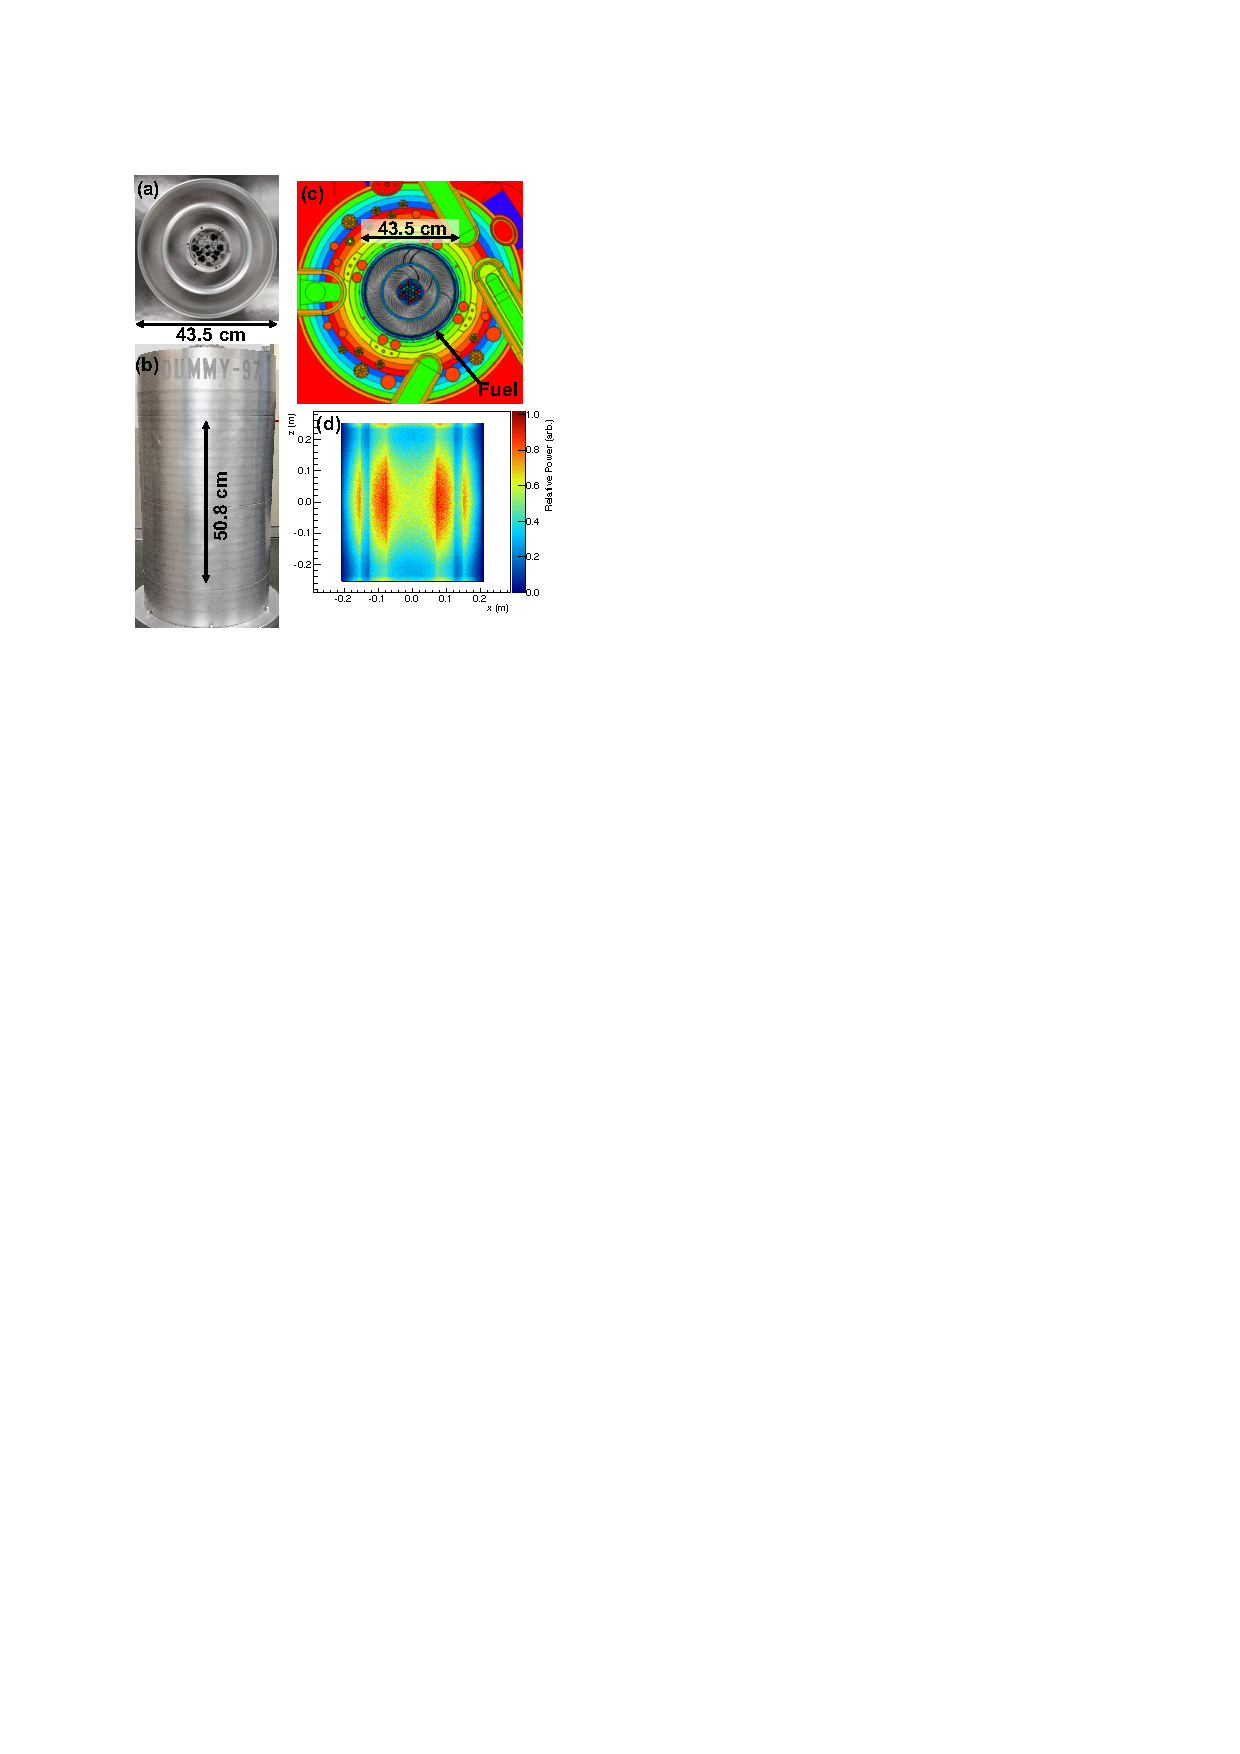
\includegraphics[width=0.5\textwidth]{Figures/HFIR.pdf}
    \caption[The dimensions and power distribution of HFIR]{A model of the reactor~\cite{bib:prospect_nim} parameters (a) and (b) are the diameter and height of the HFIR core.
    The location of the HFIR core in a detailed reactor system simulation is indicated in (c).
    (d) is a projection of the fission power density of HFIR at the x-z plane.}
    \label{fig:HFIR}
\end{figure}

    HFIR is a cylindrical fission reactor.
    Its compact size, as shown in Table~\ref{tab:HFIR} and Figure~\ref{fig:HFIR}, is ideal to limit the uncertainty of baseline.
    To maintain its high $^{235}$U enrichment, the HFIR reactor has relatively short reactor cycles.
    In this case, the fuel evolution of fissile isotopes is negligible.
    
    The HFIR facility also brought unique challenge of background for neutrino measurement. 
    Because of the very short baseline requirement of the experiment and availability of the experiment site, the PROSPECT AD is exposed to cosmic ray background with minimal overburden. 
    The detector also faces reactor correlated background, e.g. the neutron background generated from reactor and the $\gamma$ ray background from the metallic materials in the piping of the facility.
    A comprehensive background characterization is therefore organized in the research and development (R\&D) phase of PROSPECT~\cite{bib:prospect_background}. 
    The detector and additional background shielding was designed based on the by this background survey.
    
\begin{figure}
    \centering
    %\vspace{0pt}
    \includegraphics[width=0.47\textwidth, valign=t]{Figures/NeutronBGMap.pdf}
    %\vspace{0pt} 
    \includegraphics[width=0.51\textwidth, valign=t]{Figures/GammaBGMap.pdf}
    \caption[Local background distribution at HFIR facility]{(Left) The reactor correlated neutron background rate (nSv/h) shown in a map of the HFIR site where PROSPECT is deployed.
    (Right) The local $\gamma$ ray background rate (Hz) shwon in the same map.
    }
    \label{fig:prospect_background}
\end{figure}

\Section{Detector Design}

    The PROSPECT AD is a $\sim$4~ton $^{6}$Li-doped LS ($^{6}$LiLS) detector deployed at 7-9~m baselines from the HFIR core.
    The key parameters of the PROSPECT AD is shown in Table~\ref{tab:PROSPECT_AD}.
    The schematic of detector deployment at the HFIR facility is shown in Figure~\ref{fig:PROSPECT_LAYOUT}.
\begin{table}[h]
    \centering
    \caption[PROSPECT AD Parameters]{The key parameters of the PROSPECT AD~\cite{bib:prospect_nim}.}
    \begin{tabular}{cc}
    \hline
    \hline
    Parameter  & Value   \\ 
    \hline
    Target volume \& mass    & 3760 litters, 3.68 tons\\
    Target dimension & 1.176\,m wide $\times$ 2.045\,m long  $\times$ 1.607\,m tall \\
    Baseline     & 7.9~m \\
    Liquid scintillator & EJ-309 based LS with $<$0.1\% $^{6}$Li \\
    LS energy resolution & 4.5\% \\
    Segments & 14 horizontal $times$ 11 vertical \\
    Segment dimension & 1.176\,m wide $\times$ 14.5~cm long  $\times$ 14.5~cm tall \\
    Light collection & diameter = 12.7~cm (5~inch) PMTs\\
    \hline
    \end{tabular}
    \label{tab:PROSPECT_AD}
\end{table}
\begin{figure}
    \centering
    %\vspace{0pt}
    \includegraphics[width=0.6\textwidth]{Figures/Layout.pdf}
    \caption[The layout of the PROSPECT experiment]{The layout of the PROSPECT experiment.
    The PROSPECT AD is deployed 7.9~m from the reactor center to the detector center.
    Additional on site shield was installed between the reactor pool and the AD to eliminate the local $\gamma$ ray background.
    }
    \label{fig:PROSPECT_LAYOUT}
\end{figure}
    
    The anatomy of the PROSPECT AD is shown in Figure~\ref{fig:PROSPECT_AD}.
    The inner volume of detector is contained in a liquid tight acrylic vessel filled with the $^{6}$LiLS, which is made from an EJ-309 base, an organic LS \cite{bib:lspaper}.
    The designed energy resolution is 4.5\% to optimize PROSPECT's IBD spectrum measurement.
    An advantage of utilizing the EJ-309 is the pulse shape discrimination (PSD) feature making the PROSPECT AD sensitive to particle identity, which is described in detail in Section~\ref{sec:detection}.
    The $^{6}$Li is loaded as a main neutron capture isotope.

\begin{figure}
    \centering
    %\vspace{0pt}
    \includegraphics[trim = 0cm 2cm 0cm 2cm, clip,width=0.6\textwidth]{Figures/DetectorDesign.pdf}
    \caption[The design of PROSPECT AD]{The design of PROSPECT AD consisting the inner detector and the shielding.
    The inner detector includes $^{6}$LiLS, the optical grid, photomultiplier tubes (PMTs), and the calibration system.
    }
    \label{fig:PROSPECT_AD}
\end{figure}

    The inner volume of the PROSPECT AD is optically segmented by a light weight optical grid subsystem~\cite{bib:prospect_og}.
    The optical grid consist of highly reflective carbon fiber backed separators dividing the LS volume into 14$\times$11 identical longitudinal segments. 
    The ends of each segments are enclosed by two diameter = 12.7~cm photomultiplier tubes (PMTs).
    The 
    The segment with largest LS light yield is identified as the interaction point (x- and y-direction) of an incident particle.
    The readout of PMT housed in mineral-oil filled acrylic modules (PMT optical modules) on both sides of each segment, allowing for timing- and charge-based position reconstruction along the axis (z-direction) of each segment~\cite{bib:prospect_50, bib:P20}.
    Hence, the optical grid made PROSPECT AD able to reconstruct incident particles' track and 3D position, which is an essential function for the cosmic ray rejection and the oscillation measurement in the baseline between 7~m to 9~m.
    
\Section{Antineutrino Detection}
\label{sec:detection}

\Section{Optical Grid}
\label{sec:OG}

\Section{Background Shielding}

\Section{Calibration System}

\Section{Detector Construction and Commissioning}

\Section{Data Acquisition}

\Chapter{Detector Research and Development}
\label{Ch4}

The research and development (R\& D) of PROSPECT detector began in 2014.
Multiple prototypes were assembled to in the R\& D phase to develop and demonstrate a variety of detector design.
In this phase, many candidate materials were tested. 
The time line of the PROSPECT R\& D is shown in Table~\ref{tab:Prototypes}

\begin{sidewaystable}[h!]
    \centering
    \caption[PROSPECT R\& D and construction phases]{PROSPECT R\& D and construction phases.}
    \begin{tabular}{cccc}
        Phase & Time & Goal & Reference \\
        \hline
        \hline
        0.1~liter prototype  & Aug. 2014 & DAQ, LS performance &\\
        2~liter prototype   & Dec. 2014 to Mar. 2015 & Background survay, shielding & \cite{bib:prospect_background}\\
        20~liter prototype   & Mar. 2015 to Aug. 2016 & Single segment performance & \cite{bib:P20} \\
        50~liter prototype   & Jan. 2016 to Mar. 2019 & Two segment event reconstruction, detector stability & \cite{bib:P50} \\
        \hline
        LS fabrication & Jan. 2016 to Oct. 2017 & Fabrication  & \cite{bib:P50} \\
        PMT module assembly & Jan. 2016 to Mar. 2019 & Two segment event reconstruction, detector stability & \cite{bib:P50} \\
        Optical grid component fabrication & Jan. 2016 to Mar. 2019 & Two segment event reconstruction, detector stability & \cite{bib:P50} \\  
        \hline
		Detector assembly & Jan. 2016 to Mar. 2019 & Two segment event reconstruction, detector stability & \cite{bib:P50} \\       
        Detector commissioning & Jan. 2016 to Mar. 2019 & Two segment event reconstruction, detector stability & \cite{bib:P50} \\ 
        \hline 
        Data acquisition & Jan. 2016 to Mar. 2019 & Two segment event reconstruction, detector stability & \cite{bib:P50} \\ 
        \hline
    \end{tabular}
        \label{tab:Prototypes}
\end{sidewaystable}

\Section{Prototype Research}
	
\Section{Optical Grid}
\label{sec:OG}

\Section{Calibration System}

\Section{Detector Construction and Commissioning}

\Section{Data Acquisition}

\Chapter{Physics of Liquid Scintillator Detectors}
\label{Ch5}

The PROSPECT AD reconstructs event energy by collecting light produced by the $^6$LiLS.
The PMTs of PROSPECT collect optical photons (photons with visible wavelength) from scintillation light yield. 
The light yield of the $^6$LiLS in response to an incident particle is not directly proportional to energy.
Instead, complicated molecular effects in the scintillator, called Birks' quenching, causes nonlinear energy response. 
Additional nonlinear light yield is contributed from the Cherenkov radiation of charged particles with high enough energy.
It is a vital step to understand the nonlinearity of light yield in PROSPECT to reconstruct particle energies and determine the absolute energy of $^{235}$U-produced \nuebar.

\Section{Organic Scintillator Light Yield}

The $^6$LiLS of PROSPECT AD is an organic scintillator.
The fluorescence process of organic scintillators is defined by the de-excitation photons of molecules from a variety of energy levels.
Particle energy is absorbed by a scintillator molecule to excite its electron configurations.
The de-excitation photon released by the excited molecule is the light yield of an organic scintillator.
The scintillation photon yield per incident energy, referred to as scintillation efficiency, is a vital property of a specific scintillator.
In an ideal energy-light conversion, the light yield with a scintillation efficiency $S$ can be expressed as
\begin{equation}
\frac{dL}{dx} = S(\frac{dE}{dx}).
\end{equation}
However, this efficiency is usually affected by radiationless de-excitation, such as molecular thermal motion, and light absorption by impurities, such as oxygen dissolved in an organic LS .
The mechanics of energy deposition in the scintillator differs with different types of particle interactions.

\Subsection{Beta Interactions}\label{sec:511}
Electron (betas) and positrons are the main subjects measured to reconstruct the reactor neutrinos' energy.
Only a small portion of the beta particle's kinetic energy is converted to the scintillation light. 
The major beta energy absorption mechanisms are the collision with atoms in the medium and the Bremsstrahlung effect.
Collisional loss is the major contributor for lower energy betas (below 10~MeV in $^6$LiLS), where the energy loss is due to ionization and excitation of the atoms in the medium.
The Bremsstrahlung effect absorbs electron/positron energy when the coulomb forces in the medium deflect it.
The energy loss of beta particles is commonly calculated based on the material compound components with the ESTAR database~\cite{bib:estar}, as shown in Figure~\ref{fig:EStar},
where the total energy loss is
\begin{equation}
\label{eq:dedx}
\frac{dE}{dx} = (\frac{dE}{dx})_c + (\frac{dE}{dx})_r.
\end{equation}
In the range of reactor neutrino produced IBD positron energy (0, 10) MeV, the major contributor of the positron energy loss is collisional loss. 
Because of the stopping power of the scintillator of PROSPECT, the length of the positron path is limited to a scale of several centimeters.

\begin{figure}[h!]
    \centering
    \includegraphics[width=0.7\textwidth]{Figures/ESTAR.png}\\
    \caption[Electron energy loss in $^6$LiLS]{The electron $dE/dx$ through $^6$LiLS calculated by E-star~\cite{bib:estar}.
    When electron energy is higher ($> 10$~MeV), the Brestrahlung effect contributes more significantly.}
    \label{fig:EStar}
\end{figure}

\Subsection{Muon Interactions}
Interactions absorbing the energy of cosmic muons is similar to beta particle interactions. 
Due to its high kinetic energy and mass-to-charge ratio, a cosmic muon can travel through multiple segments of the PROSPECT AD.
Occasionally, a Michel electron is generated when a muon decays inside of the detector volume.

\Subsection{Gamma Ray Interactions} 
Two gamma rays, each with 0.511~keV energy, are generated from the annihilation of an IBD positron.
The annihilation gamma events are part of the IBD prompt event along with positron kinetic energy deposition as described in Section~\ref{sec:511}.
Gamma energy is also utilized in energy scale calibration for PROSPECT.
Gamma interaction channels in scintillator include a photoelectric effect, Compton scattering, and electron-positron pair production.

Due to the photoelectric effect, gamma energy is partially absorbed by atoms in the medium.
Photo electrons (PEs) are emitted in the process when gamma energy overcomes the binding energy of the electron at its original shell. 
A PE's energy generally ranges from the scale of 1~keV to 10~keV.
The photoelectric effect is the major contributor causing energy loss of gamma rays with energy below 0.1~MeV.
If a single energy gamma loses all of its energy through photoelectric absorption, its energy deposition in a large detector volume would be a delta function.

The Compton scattering of a gamma photon also emits free electrons in the medium. 
The energies of the scattered electron and gamma are dependent on the scattering angle. 
Thus, the Compton recoil electron energy is a continuous spectrum for a single energy gamma-ray input.
The maximum energy of the Compton recoil electron is obtained when the scattering angle is maximized.
The energy difference between the incident gamma photon and the Compton recoil electron is given by
\begin{equation}
E_C \equiv E_\gamma  - E_{e^-} (\theta = \pi) = \frac{E_\gamma}{1+2E_\gamma/m_e}.
\end{equation}
The cross-section of Compton scattering as a function of the scattering angle is dependent on the medium's electron structure and density. 

When the energy of the incident gamma exceeds the 1.022~MeV energy threshold, the electron-positron pair production reaction can occur among the gamma ray interactions. 
Ideally, the total energy of the electron and positron pair equals the gamma energy.
The probability of pair production varies with respect to the absorber's atomic numbers.

The photoelectric effect mainly absorbs gamma energies below 0.1~MeV. 
When the energy of a gamma-ray exceeds the pair production threshold, pair production becomes a major cause for gamma energy loss in the higher energy range. 
The Compton scattering cross-section varies with gamma energy but becomes the most significant contributor of gamma energy absorption between 0.1~MeV to 10~MeV.
Hence, Compton scattering is the major cause of gamma energy loss in PROSPECT's IBD measurement.
Despite the type of interaction, a gamma photon energy is measured through its interaction generating electron and positrons.
Therefore, the PSD signature and the detector response to a gamma-ray is similar to a beta particle, with the exception that gamma-ray energy deposition spreads significantly farther in distance than an MeV-scale beta in organic scintillator.

\Subsection{Heavy Nucleon Interactions}
As described in Chapter~3, PROSPECT relies on the $n$-$^6$Li capture interaction to tag IBD event candidates. 
The alpha particle and triton products of the $n$-Li capture lose their energy as charged particles.

Charged heavy particle energy is absorbed through coulomb force interactions.
When charged nucleons enter media, the coulomb force between the nucleons and orbital electrons excites the electrons to higher energy states or ionizes the atom.
Thus, alpha particles, tritons, and protons excite scintillator molecules similar to electrons and positrons. 
For a 1~MeV scale charged nucleon, the energy loss $dE/dx$ is significantly higher because of the higher cross-section for ionization and collision with atoms.

Unlike particles described previously, neutrons do not deposit energy through ionization directly due to its neutral electrical charge.
Therefore, the neutron energy loss mechanism is dominated by interactions with charged particles.
In particular, fast neutrons can transfer kinetic energy to a proton, alpha particle or nucleus in the medium, causing a recoil of charged heavy particles.
During recoil interactions, fast neutrons are slowed down and eventually lose most of their kinetic energy.
The inelastic scattering between a neutron and another nucleus transfers neutron energy to the nucleus, which de-excites by emitting a gamma photon.
Thermal neutrons, with kinetic energy less than 0.025~eV, can be captured by proton-abundant atoms like hydrogen, boron, and lithium with high probability. 
Typical products of neutron capture are isotopes in excited states. 
De-excitation gamma photons from the product isotopes can be detected.
In the case of the $n$-Li capture process, an alpha particle and a Triton are generated.

\Section{Birks' Quenching}

A scintillator's light yield is ideally proportional to the energy loss as in Eq.~\ref{eq:dedx}.
In reality, the quenching effect in an organic scintillator causes nonlinear light yield with respect to the energy deposition.
Multiple factors affect the quenching effect, including radiationless molecular movements and the impurities in components absorbing the energy of scintillation light.
A semi-empirical light yield conversion was developed by Birks~\cite{bib:birks, bib:birksbook}. 
This conversion is referred to as Birks' Law, which is based on experimental measurement of organic scintillators' light yields and the theoretical assumption that the quenching effect varies with incident event ionization density. 
Birks' Law of scintillator quenching is expressed as
\begin{equation}
\frac{dL}{dx} = \frac{S\frac{dE}{dx}}{1+k_{B1}\frac{dE}{dx} + k_{B2}(\frac{dE}{dx})^2},
\end{equation}
where $k_{B1}$ and $k_{B2}$ are the first and second order Birks' constants that vary for different scintillators.
Nonlinearity of light yield is severe at lower energies near the Bragg peak of the concerned particle. 

Birks' Law also indicates significantly lower light yield from incident particles with high $\frac{dE}{dx}$.
Thus, the effective light yield efficiency from protons and alpha particles is generally lower than electrons and gamma photons, resulting in severe differences between experiment-reconstructed energy and the actual deposited energy.
The reconstructed energy is hence referred to as MeV electron equivalent (MeVee).
For instance, the total energy of the alpha particle and Triton from $n$-Li capture is 4.78~MeV, while its PROSPECT detector reconstructed energy is $\sim$0.55~MeVee.
The nonlinear scintillation response to different particles with various energy is shown in Figure~\ref{fig:birks}.

\begin{figure}[h!]
    \centering
    \includegraphics[width=0.55\textwidth]{Figures/BirksNonlinearHigh.pdf}
    \includegraphics[width=0.38\textwidth]{Figures/BirksNonlinearLow.pdf}
    \caption[Quenched scintillator light response]{
     (Left)The nonlinear scintillator response to different particle types~\cite{bib:birks}.
	(Right) The light response of a scintillator to low energy electrons.
    $S$ is the light signal output of Birks' measurement with organic scintillator anthracene.
    Because of high $dE/dx$, protons and alpha particles produce significantly less scintilation light per MeV, compared to an electron.
    }
    \label{fig:birks}
\end{figure}

Different scintillators have unique sets the Birks' quenching constants $k_{B1}$ and $k_{B2}$.
Measurements of $k_{B1}$ and $k_{B2}$ are usually made by comparing the electron and heavy-ion light yields at constant incident energy.
However, the measured quenching constants are particularly challenging to simulate in most experiments due to large uncertainty of $dE/dx$ calculation in MC simulations.
The method used in PROSPECT simulations is discussed in Chapters~\ref{Ch6} and \ref{Ch7}.

\Section{Cherenkov Radiation}
Photons produced through Cherenkov radiation~\cite{bib:ckov} are another source of light in PROSPECT.
When a charged particle's speed in a medium is higher than the phase speed of light, a Cherenkov photon is emitted as the polarizable medium molecules are polarized by the charged particle.
Coherent light is radiated at an angle with respect to the particle's traveling direction and speed.
The number of photons generated in Cherenkov radiation is 
\begin{equation}
    \frac{d^2N}{dxd\lambda} = \frac{2\pi\alpha z^2}{\lambda}\left(1- \frac{1}{\beta^2n^2(\lambda)}\right),
\end{equation}
where $N$ is number of photons, $\alpha$ is the fine structure constant, $z$ is the particle's electric charge, $\beta$ is the speed of the particle, and $n(\lambda)$ is the index of refraction of the medium.
The actual optical spectrum of the Cherenkov light is dependent on the scintillator index of refraction, transmission efficiency, and absorbance.
The thresholds of Cherenkov radiation production for electrons and gammas are shown in Figure~\ref{fig:ckovthresh}, where the threshold for electrons is $\sim$0.2~MeV when the medium index of refraction is 1.5.

\begin{figure}[h!]
    \centering
    \includegraphics[width=0.5\textwidth]{Figures/CkovThresh.pdf}
	\caption[Cherenkov radiation thresholds]{
    The Cherenkov radiation thresholds of gammas and electrons in media with different indices of refraction.}
    \label{fig:ckovthresh}
\end{figure}

Cherenkov radiation of charged particles produce prompt photons in the PROSPECT AD that is indistinguishable from scintillation light.
The nonlinear energy response caused by Cherenkov radiation is discussed in Chapters~\ref{Ch6} and \ref{Ch7}.


\Chapter{Monte-Carlo Simulations for PROSPECT}
\label{Ch6}

In PROSPECT's reactor neutrino measurement, Monte-Carlo simulation (MC) is necessary to 
\begin{itemize}
	\item Test detector configurations during R\&D
	\item Characterize detector performance
	\item Study detector energy response to a variety of particles
	\item Determine systematic uncertainties of detector geometry and light response
	\item Generate spectrum models and toys for parameter searches and sensitivity studies
\end{itemize}
PROSPECT-G4 (PG4) is the PROSPECT customized MC simulation package programmed based on the Geant-4~\cite{bib:geant4} toolkit.
This simulation package allows users to adjust detector geometries and material properties to provide important information guiding detector design. 
PG4 was developed with prototype detectors; and was used to demonstrate the simulation's reproduction of calibration data.
Because of limitations in computing resources and time, PG4 contains necessary simplifications in its description of PROSPECT's detector geometry and particle interactions.
Adjusting PG4's simulation of detector geometry, particle generation functions, and energy response is one of the essential parts in my thesis research.

\Section{Geometrical Simulation}

PROSPECT detector configurations are simulated in PG4. 
The simulated structures include $^6$LiLS, the optical grid, PMT modules, containers, and shielding.
Although most of the materials utilized in the PROSPECT AD are saved in Geant4 material databases with their chemical components and densities, $^6$LiLS is customized in PG4 by characterizing the density, chemical components, and doping percentage of the scintillator.
The simulated $^6$LiLS is composed of 0.9781~g/cm$^3$ density EJ-309, which is composed of 84.14\% C, 9.52\% H, and 6.34\% O by weight.
Additional water and LiCl solution was added with the concentration easily adjustable in simulation.
The reflectances of the optical grid separators are set based on direct optical measurements described in Chapter~\ref{Ch4}.

Some approximations was made to simplify the programming and running of PG4.
The DAQ cables and systems are not included in the simulation because they do not contribute dead volume to the active detector volume.
For simplicity of programming, the separator pinching tabs of PLA rods are continuous from end to end along each cell.
The separator materials consist of only FEP films, and carbon fibers, as the density and chemical components of other laminated materials are not known.

For the radioactive calibration system, only calibration source capsules are simulated in PG4; the source driving components have minimal affect on dead volume in the detector. 
The source capsule materials and dimensions are programmed according to the actual design.

The on-site shielding wall and the detector shielding walls are also simulated based on the designed material and dimensions.

\Section{Particle Generation and Interaction Simulations}

Because of neutrinos' low IBD cross-section, direct neutrino simulation is not realistic in PG4. 
Instead, IBD produced positrons and neutrons are generated to mimic the IBD interaction in the detector. 
In PG4 simulation, each IBD event contains a positron-neutron pair generated from the same vertex with their sum of energy equal to a user defined neutrino energy plus a rest proton energy (the IBD total energy).
The IBD total energy and vertex position can be adjusted for different analysis purposes, including model generation, detector response studies and uncertainty calculations.
In the special case of simulating the reactor neutrinos generated from HFIR, IBD total energies are generated based on the Huber model of the reactor neutrino spectrum~\cite{bib:huber}.
As the reactor location is approximately 45$^\circ$ below the PROSPECT detector, the angular distribution of the IBD products is implemented as shown in Figure~\ref{fig:IBDangle}.

\begin{figure}[h!]
    \centering
    \includegraphics[width=0.7\textwidth]{Figures/IBDKinematics.pdf}
	\caption[The simulated IBD products angular distribution]{
    The simulated IBD products' angular distributions, with red dots representing positrons and blue dots representing neutrons.}
    \label{fig:IBDangle}
\end{figure}

Radioactive sources utilized in calibration are simulated in PG4 with custom built particle generators. 
The gammas and electrons of the calibration sources are generated from user defined vertexes with energies extracted from the energy levels and transition probabilities saved in the ENSDF database~\cite{bib:ENSDF}. 
For the $^{252}$Cf spontaneous fission neutron source, the emitted neutrons and gammas from its fission reaction are simulated instead of directly simulating the fission process. 

The cosmic ray background is simulated with the external cosmic ray shower generator CRY~\cite{bib:CRY}.

\Section{Truth-level Simulation}

Identification of particle type (PID) of PG4 is consistent with Geant4, which uses PDGID~\cite{bib:PDG} of particles.
In the case of neutron capture events, the $A$ and $Z$ values of the neutron capturing atoms are recorded.

Particle energy depositions and positions in the detector are tracked with the \texttt{G4Track} and \texttt{G4Step} objects, as illustrated in Figure~\ref{fig:g4step}.
\texttt{G4Track} is a snapshot of a particle.
Every two points in \texttt{G4Track} are connected by \texttt{G4Step}.
Every two steps are separated by 1) a particle interaction, 2) particle traversal through the boundary of two geometrical volumes in Geant4, 3) a particle traveled the maximum length of each step, 4) a particle stops or exits the simulation world volume.
\texttt{G4Track} saves the particle's PID, energy, and position information.
\texttt{G4Step} saves the particle's energy loss from the beginning to the end of a step.
Therefore, a particle's energy deposition in each segment of the PROSPECT AD can be saved by summing the the energy deposits in all steps in a segment. 
Each \texttt{G4Step}'s maximum length is set by user.
The step size is independent of particle energy and current medium.
As a result, the $dE/dx$ calculated in each step does not precisely reflect actual material stopping power.
\begin{figure}[h!]
    \centering
    \includegraphics[width=0.8\textwidth]{Figures/G4Step.pdf}
	\caption[Illustration of PG4 event tracking]{
    An illustration of PG4 event tracking, where an arbitrary is recorded. 
    The yellow dots and the arrows connecting among them represent \texttt{G4Track}s and \texttt{G4Step}s.
    }
    \label{fig:g4step}
\end{figure}

PG4's ability to track a particle's energy loss step-by-step enables simulation of nonlinear detector response. 
In Chapter~\ref{Ch5}, the Birks' quenching function is determined as 
\begin{equation}
\frac{dL}{dx} = \frac{S\frac{dE}{dx}}{1+k_{B1}\frac{dE}{dx} + k_{B2}(\frac{dE}{dx})^2}.
\label{eq:birkslaw}
\end{equation}
Using the $dE/dx$ calculated by each step, the quenched light yield can be effectively expressed as the reduction of energy deposition 
\begin{equation}
   \frac{dE_{quench}}{dx} = \frac{\frac{dE}{dx}}{1+k_{B1}\frac{dE}{dx}+k_{B2}(\frac{dE}{dx})^2}.
\end{equation}
Hence, the quenched energy of a particle is
\begin{equation}
   E_{quench} = \sum_{i}^{steps}\frac{\frac{dE_i}{dx}}{1+k_{B1}\frac{dE_i}{dx}+k_{B2}(\frac{dE_i}{dx})^2}, 
   \label{eq:birksMC}
\end{equation}
where $k_{B1}$ and $k_{B2}$ are effective Birks' constants, since the $dE/dx$ calculated in each \texttt{G4Step} differs from actual material stopping power.
PG4's simulation of Birks' quenching is a unique approach in particle detector simulation.
It allows the user to adjust the detector's nonlinear response by changing the quenching factors ($k_{B1}$ and $k_{B2}$ ) of the simulated detector.
This is a necessary simulation feature because the event reconstruction for the segmented PROSPECT AD is complicated, as discussed in Chapter~\ref{Ch8}.

Cherenkov radiation can also be simplified using the energy loss and speed of particles calculated by PG4.
Because of limited computing resources, optical photon simulation for high energy interactions is unrealistic.
As discussed in Chapter~\ref{Ch5}, the number of photons generated as Cherenkov radiation is expresssed as 
\begin{equation}
    \frac{d^2N}{dxd\lambda} = \frac{2\pi\alpha z^2}{\lambda}\left(1- \frac{1}{\beta^2n^2(\lambda)}\right).
\end{equation}
By learning the detector's light transmission spectrum and wavelength shifting efficiency, the optical spectrum of the Cherenkov photon can be used to calculate additional light collection from it.
An effective Cherenkov photon contributed energy $E_c$ can be added to the effective energy in PG4,
\begin{equation}
E_{c} = k_{c}\sum_{\lambda}N_\lambda E_\lambda,
\end{equation}
where $E_\lambda$ is the energy contributed by each photon, $k_c$ is an effective \textit{Cherenkov energy} coefficient.
The contribution of $E_{c}$ to the reconstructed energy is adjustable by the user in energy response studies as discussed in Chapter~\ref{Ch8}.

\Section{DAQ Pulse Simulation}

The MC output of the PG4 simulation is converted to files with structures identical to actual PROSPECT data.
The purpose of this conversion is to force MC simulation to be consistent with detector responses at different times, because the evolution of detector response over time has been observed.
The structure of the PG4 MC output and the actual PROSPECT data are shown in Figure~\ref{fig:MCstructure}.
A PG4 MC output contains primary particles and particle interactions, where the `ionization event' saves the energy deposition and timing information in each segment. 
The `neutron capture' category is set to save the neutron interaction, especially the neutron-atom interaction to record the neutron capture events and the interactions related to the events.
The low level PROSPECT `detector pulse data' saves the ADC timing and channel information.
The `physics data', also referred to as high level data, saves the event position, time, reconstructed energy and PID information based on calibration and analysis of the low level pulse data.
These data processing and calibration procedure is discussed in Chapter~\ref{Ch7} and \ref{Ch8}.

\begin{figure}[h!]
    \centering
    \includegraphics[width=0.8\textwidth]{Figures/MCStructure.pdf}\\
    \includegraphics[width=0.5\textwidth]{Figures/PulseStructure.pdf}
	\includegraphics[width=0.4\textwidth]{Figures/PhysStructure.pdf}\\
	\caption[The data structure of MC simulation and PROSPECT data]{
	A schematic of the data structure of MC simulation and the actual PROSPECT data. 
	(Top) The structure of PG4 output, where the recorded categories share same event IDs.
	(Bottom left) The low level DAQ pulse data from unpacking the raw data. 
	(Bottom right) The high level physics data of the PROSPECT AD calibrated from the DAQ pulse data. 
    }
    \label{fig:MCstructure}
\end{figure}

The PG4 output is converted to simulated pulse and physics data through energy-ADC pulse conversion, which is a reversed conversion of the usual detector calibration, as shown in Figure~\ref{fig:MCconversion}.
PROSPECT's detector response information at different times, consisting the light response, DAQ gain setting, and PSD distributions, is saved in the PROSPECT calibration database. 
The MC energy deposition is converted to ADC channels based on this PROSPECT calibration database.
The calibration database saves ADC-energy calibration values with respect to time, and the template pulse shapes of different particles at each PMT channel.
Hence, the MC events can be converted to the simulated pulse data with PSD values, PMT pulses, and event time coincidences with time and position variations taken into consideration. 
The simulated pulse data can be calibrated to obtain simulated physics data, which is discussed in Chapter~\ref{Ch7}.
These procedures ensure precise detector response simulation even in the presence of non-uniformity and time-variation of the detector response.

\begin{figure}[h!]
    \centering
    \includegraphics[width=0.9\textwidth]{Figures/MCconversion.pdf}\\
	\caption[Schematic of PG4 output conversion]{
	A schematic of PG4 output conversion procedures.
    }
    \label{fig:MCconversion}
\end{figure}

\Chapter{Prompt Energy Spectrum of Antinetrino from $^{235}$U}


\Chapter{Prompt Energy Spectrum of Antinetrino from $^{235}$U}
\label{Ch8}

\Section{IBD Event Selection}

\Section{The Observation of Reactor Neutrino on Earth Surface}

\Section{Background Analysis}

\Section{Signal Stability}

\Section{Prompt Energy Spectrum}

\Section{Comparison with Spectrum Models}



\bibliographystyle{ieeetr}
\bibliography{reference}

\end{document}
